\documentclass[11pt,a4paper]{article}
\usepackage{fontspec}
\setmainfont{TeX Gyre Pagella}
\newfontfamily\headfont{Inter}[UprightFont=*-ExtraBold,BoldFont=*-ExtraBold,Extension=.otf,Path=/usr/share/fonts/opentype/inter/]
\usepackage[a4paper,margin=2.3cm]{geometry}
\usepackage{graphicx,booktabs,float,caption,array,xcolor,longtable}
\usepackage{xurl}
\usepackage[hidelinks]{hyperref}
\usepackage{titlesec}
\usepackage[round]{natbib}
\usepackage{setspace}
\setstretch{1.05}
\renewcommand{\topfraction}{0.9}
\renewcommand{\bottomfraction}{0.8}
\renewcommand{\textfraction}{0.1}
\renewcommand{\floatpagefraction}{0.75}
\setlength{\parindent}{0pt}
\setlength{\parskip}{0.55em}
\titleformat{\section}{\headfont\Large}{\thesection}{0.8em}{}
\titleformat{\subsection}{\headfont\large}{\thesubsection}{0.8em}{}
\captionsetup{font=small,labelfont=bf}
\urlstyle{same}
\hypersetup{pdftitle={Where Every Film Was Shot},pdfauthor={Tristan Hotham}}


\begin{document}
\begin{center}
{\Large\bfseries Where Every Film Was Shot\par}
\vspace{0.4em}
{\large Filming locations of 23,468 films in Wikidata:\\film cities, foreign productions and the James Bond films\par}
\vspace{1.2em}
{\large Tristan Hotham\par}
\vspace{0.3em}
{\small Independent researcher\\
ORCID: 0000-0003-4931-9349\\
DOI: \href{https://doi.org/10.5281/zenodo.23847354}{https://doi.org/10.5281/zenodo.23847354}\par}
\vspace{0.8em}
2026
\end{center}

\begin{quote}
\small
\begin{center}\textbf{Abstract}\end{center}
Films are often shot somewhere other than where they come from or where they are set. I use Wikidata, the open knowledge base behind Wikipedia, to map the filming locations of every film it records with a located filming place: 23,468 films, 7,926 locations and 35,108 film-location pairs. Because 20\% of those pairs name only a whole country and 14\% only a state or region, I classify each location by level and map only cities, towns and sites, so that country centroids do not appear as filming hotspots. Grouping places with the nearest large city, Los Angeles (1,514 films), New York (1,350), London (1,118) and Paris (933) lead; Pinewood Studios is the single most used site (645 films). Comparing each location's country with the film's countries of origin, 19\% of films were shot at least partly abroad. Canada hosts the most foreign productions (717, 95\% of them American), while in Malta, Morocco, Bulgaria and Iceland foreign films are the large majority of all recorded filming. The share of films shot abroad rose from 20\% in the 1950s to 25\% in the 2000s (excluding Indonesia). The 25 Eon James Bond films have 248 recorded locations in 36 countries and territories, but recent films are far better documented than early ones. Coverage is strongly biased towards American and well-known films: 40\% of films are American, and the most popular films have nearly three times as many recorded locations as the least known.

\textbf{Keywords:} film; filming locations; runaway production; film geography; James Bond; Wikidata; open data; mapping
\end{quote}

\section{Introduction}
Where a film is shot is an economic decision as much as an artistic one. Studios cluster in a few production centres, and since the 1950s producers have followed lower costs, tax incentives, skilled crews and landscapes to other countries, a pattern known in the United States as runaway production \citep{miller,goldsmith}. Some places, Toronto, Budapest, Malta or the Moroccan desert, have built industries on standing in for somewhere else \citep{scott}.

That geography is usually studied through case studies, trade data or production surveys. Wikidata \citep{wikidata} offers another, open view: it records a filming location (property P915) with coordinates for tens of thousands of films, together with each film's release dates and countries of origin. This paper uses one query of that record to ask four questions. Which places are filmed most? Which countries host other countries' productions, and has that changed by decade? Which cities are filmed mostly by foreign productions? And how do the James Bond films, the archetypal globe-trotting series, look in the data? An interactive map accompanies the paper (\url{https://maps.tristanhotham.com/film-locations/}).

The contribution is descriptive, and the main finding about the data is its unevenness. I am explicit about coverage throughout: the record is a map of documented filming, not of filming.

\section{Data}
The data come from one QLever \citep{qlever} query of Wikidata in 2026: every item that is an instance of film (Q11424) with a filming location that has coordinates (P625), with the film's English label, publication dates (P577), countries of origin (P495) and number of sitelinks, and each location's label, coordinates and country (P17). The result has 119,808 rows, because a film repeats for every combination of date, origin and location country. Table~\ref{tab:pipe} shows how this reduces to films and locations. Country outlines, first-level divisions and populated places come from Natural Earth \citep{naturalearth}.

\begin{table}[tbp]\centering\small\caption{From query to data.}\label{tab:pipe}\begin{tabular}{p{9.8cm}r}\toprule Step & Count\\\midrule
Rows returned by the query & 119,808\\
Films & 23,468\\
\quad with a year & 22,271\\
\quad with a country of origin & 23,240\\
\quad with at least one city, town or site (mapped) & 14,901\\
Filming locations & 7,926\\
\quad countries / regions / cities and towns / sites & 151 / 465 / 891 / 6,419\\
Film-location pairs & 35,108\\
\quad naming a country / region / city or town / site & 6,926 / 5,038 / 13,094 / 10,050\\
\bottomrule\end{tabular}\end{table}

\section{Methods}
\subsection{Records}
I keep one record per film and per location. A film's year is its earliest publication year; 22,271 films have one. 1,979 have no English label and are identified by their Wikidata ID. Directors (P57), from a second query, are used only for labels on the interactive map.

\subsection{Location levels}
Each location is assigned a level. It is a \emph{country} if its Wikidata ID is that of a Natural Earth country, a UK nation, a former state or a continent; a \emph{region} if it is a Natural Earth first-level division (matched by Wikidata ID or by name within the same country) or one of a short list of large named areas (French and Italian regions, big islands); a \emph{city or town} if its English label matches a Natural Earth populated place within 40 km; otherwise a \emph{site}, which includes studios, streets, buildings, parks, villages and small islands. Small territories under 1,500 km$^2$ (Hong Kong, Malta, Monaco, Singapore and others) count as cities, because their centroid is close to everywhere in them. Country and region locations are counted in all country-level figures but are never mapped as points. A location's country is the present-day country its point falls in.

\subsection{Home and abroad}
A film is shot abroad at a location if the location's country is not one of the film's countries of origin. Co-productions are at home in every partner country; films of the Soviet Union, Yugoslavia and Czechoslovakia are at home in any successor state; and crown dependencies and overseas territories count as home for the United Kingdom, the United States, France, the Netherlands and Denmark. 228 films with no country of origin are excluded. Indonesia needs separate treatment: 3,017 films (13\% of all) list the single location ``Indonesia'', 99\% of them Indonesian, so I report shares both with and without Indonesian films.

\subsection{Film cities and popularity}
For city rankings, every city, town or site is grouped with the nearest Natural Earth populated place of at least 250,000 people within 32 km, so that Pinewood Studios counts for London and Santa Monica for Los Angeles. Popularity is the number of Wikidata sitelinks (Wikipedia articles in any language and other Wikimedia pages), a rough measure of how widely a film is known. Popularity-weighted counts sum the sitelinks of the films at a place.

\subsection{James Bond}
The 25 official films made by Eon Productions, from Dr.\ No (1962) to No Time to Die (2021), were identified by a hand list of Wikidata IDs, each checked against title and year. The 1967 Casino Royale, not an Eon production, is excluded.

\section{Results}
\subsection{Where films are shot}
Figure~\ref{fig:world} shows the 14,901 films with at least one mapped place (63\% of all). The pattern is dense in western Europe and the United States, thinner across Asia and Latin America, and almost empty across Africa, a first indication of coverage.

\begin{figure}[tbp]\centering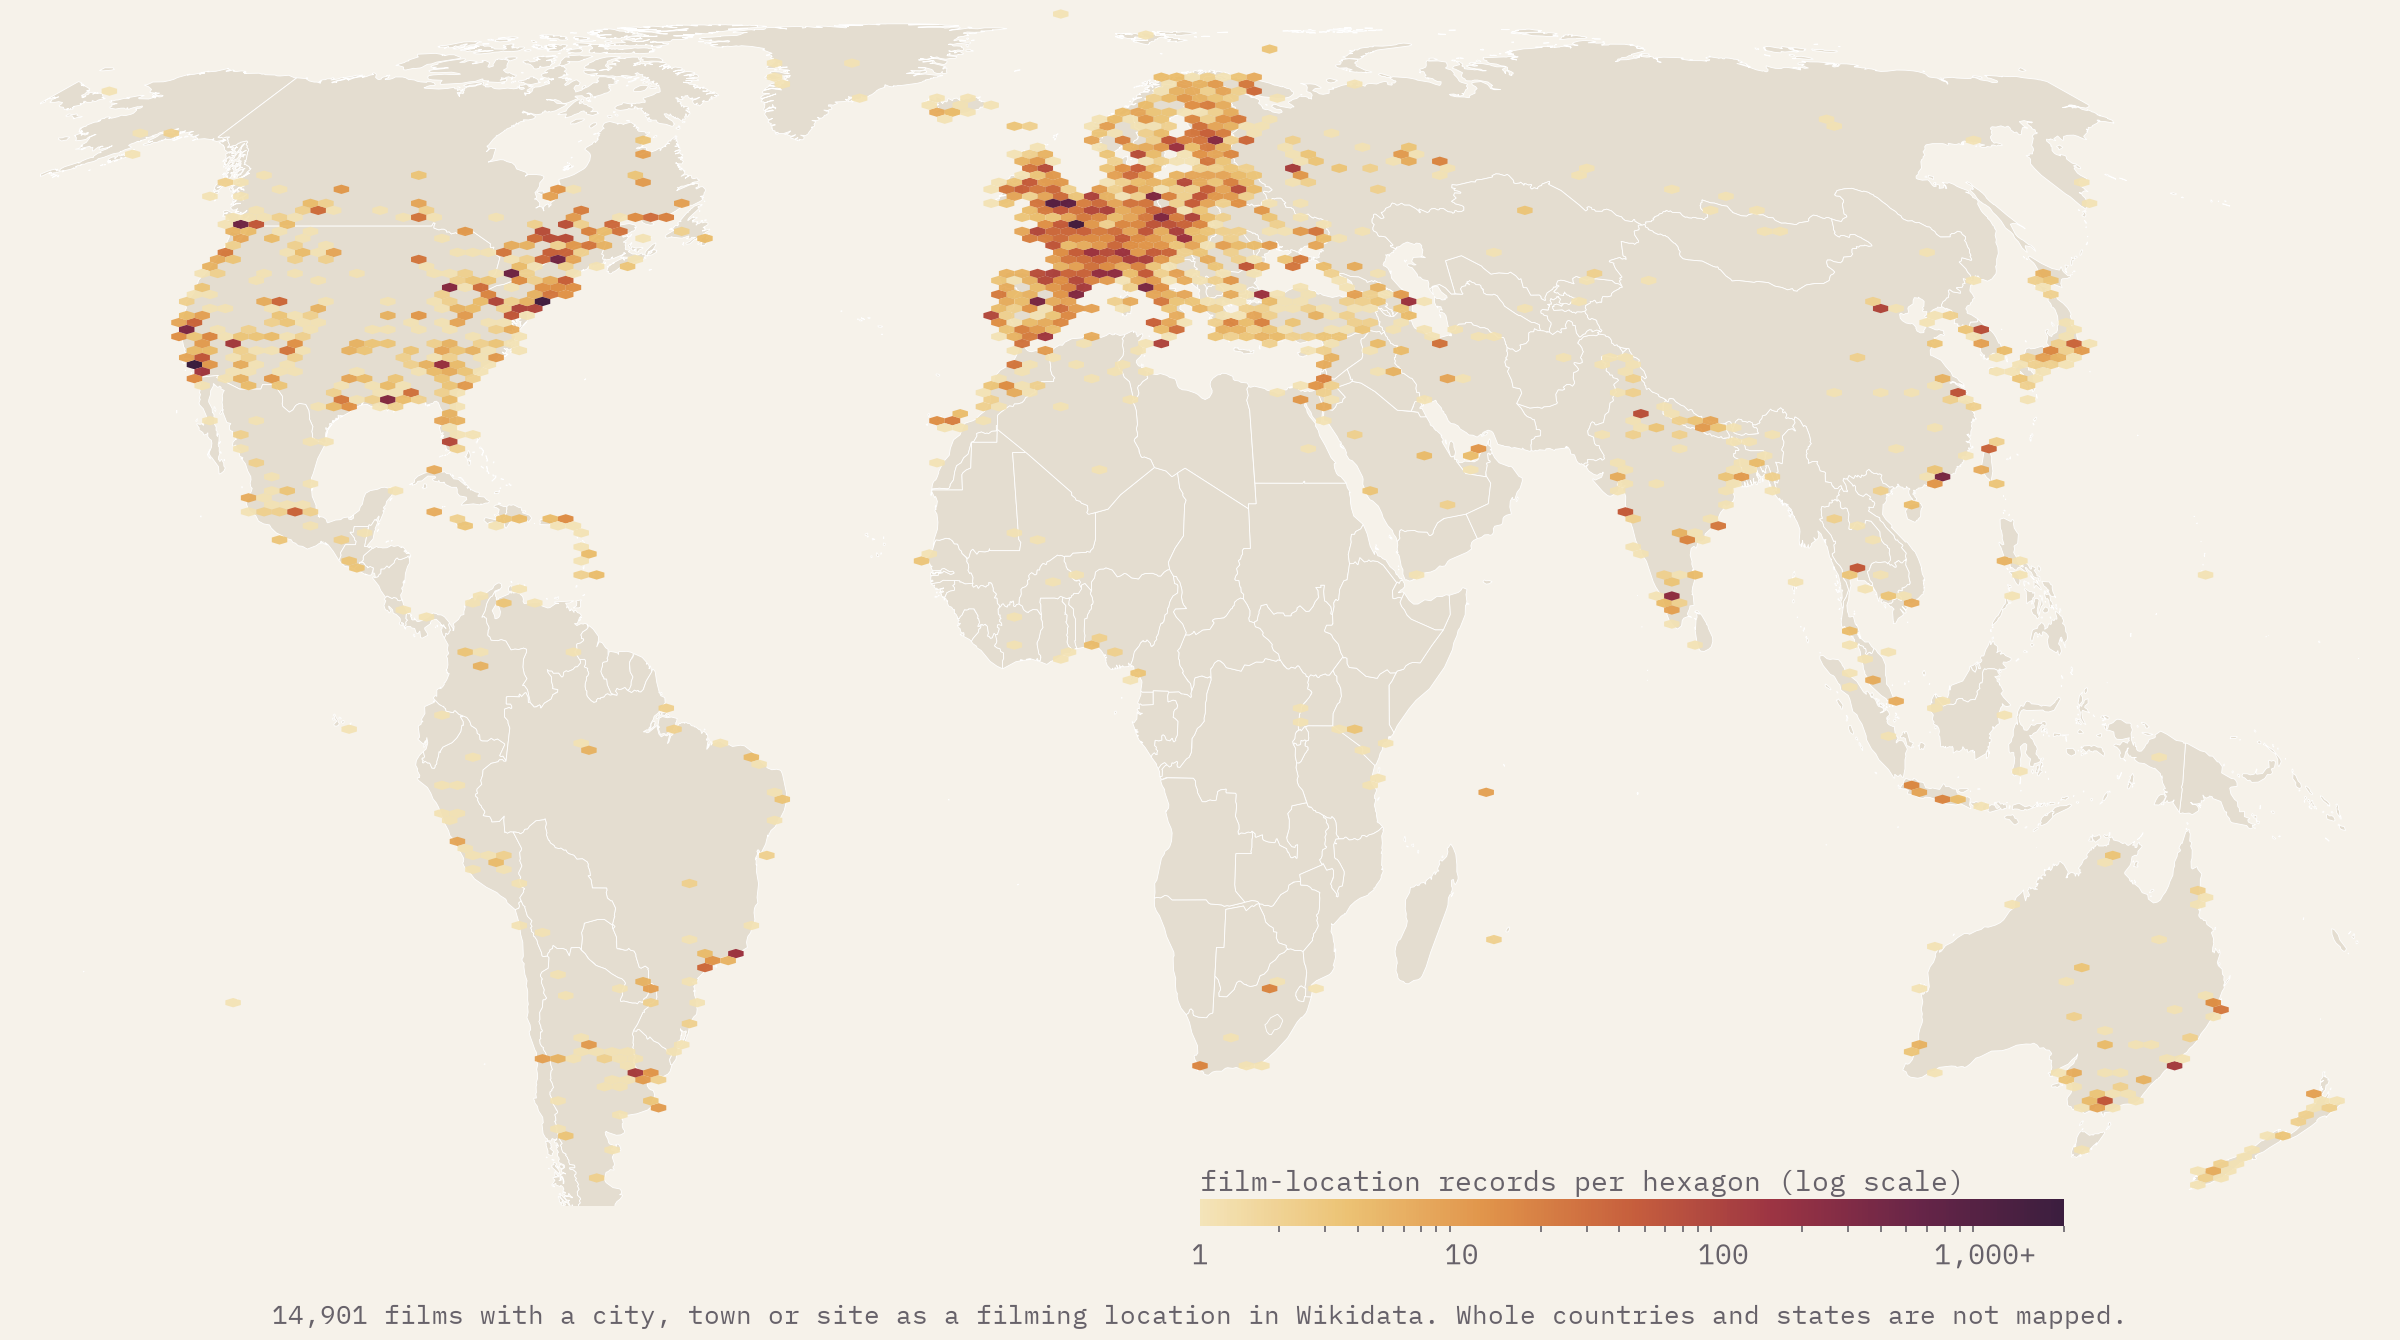
\includegraphics[width=\textwidth]{f_world.png}
\caption{Filming locations in Wikidata: film-location records per hexagon (cities, towns and sites only), Equal Earth projection.}\label{fig:world}\end{figure}

Grouped into cities (Figure~\ref{fig:cities}), Los Angeles has 1,514 films, New York 1,350, London 1,118, Paris 933 and Vancouver 452; the top five account for 34\% of films with a mapped place. Weighting by popularity leaves the top five unchanged but moves places further down: Long Beach rises from 23rd to 9th, while Hong Kong falls from 7th to 17th and Ooty, a hill town in Tamil Nadu with 199 almost entirely Indian films, to 44th. The most used single site is Pinewood Studios (645 films); 66 locations are named as studios or stages and appear 881 times.

\begin{figure}[tbp]\centering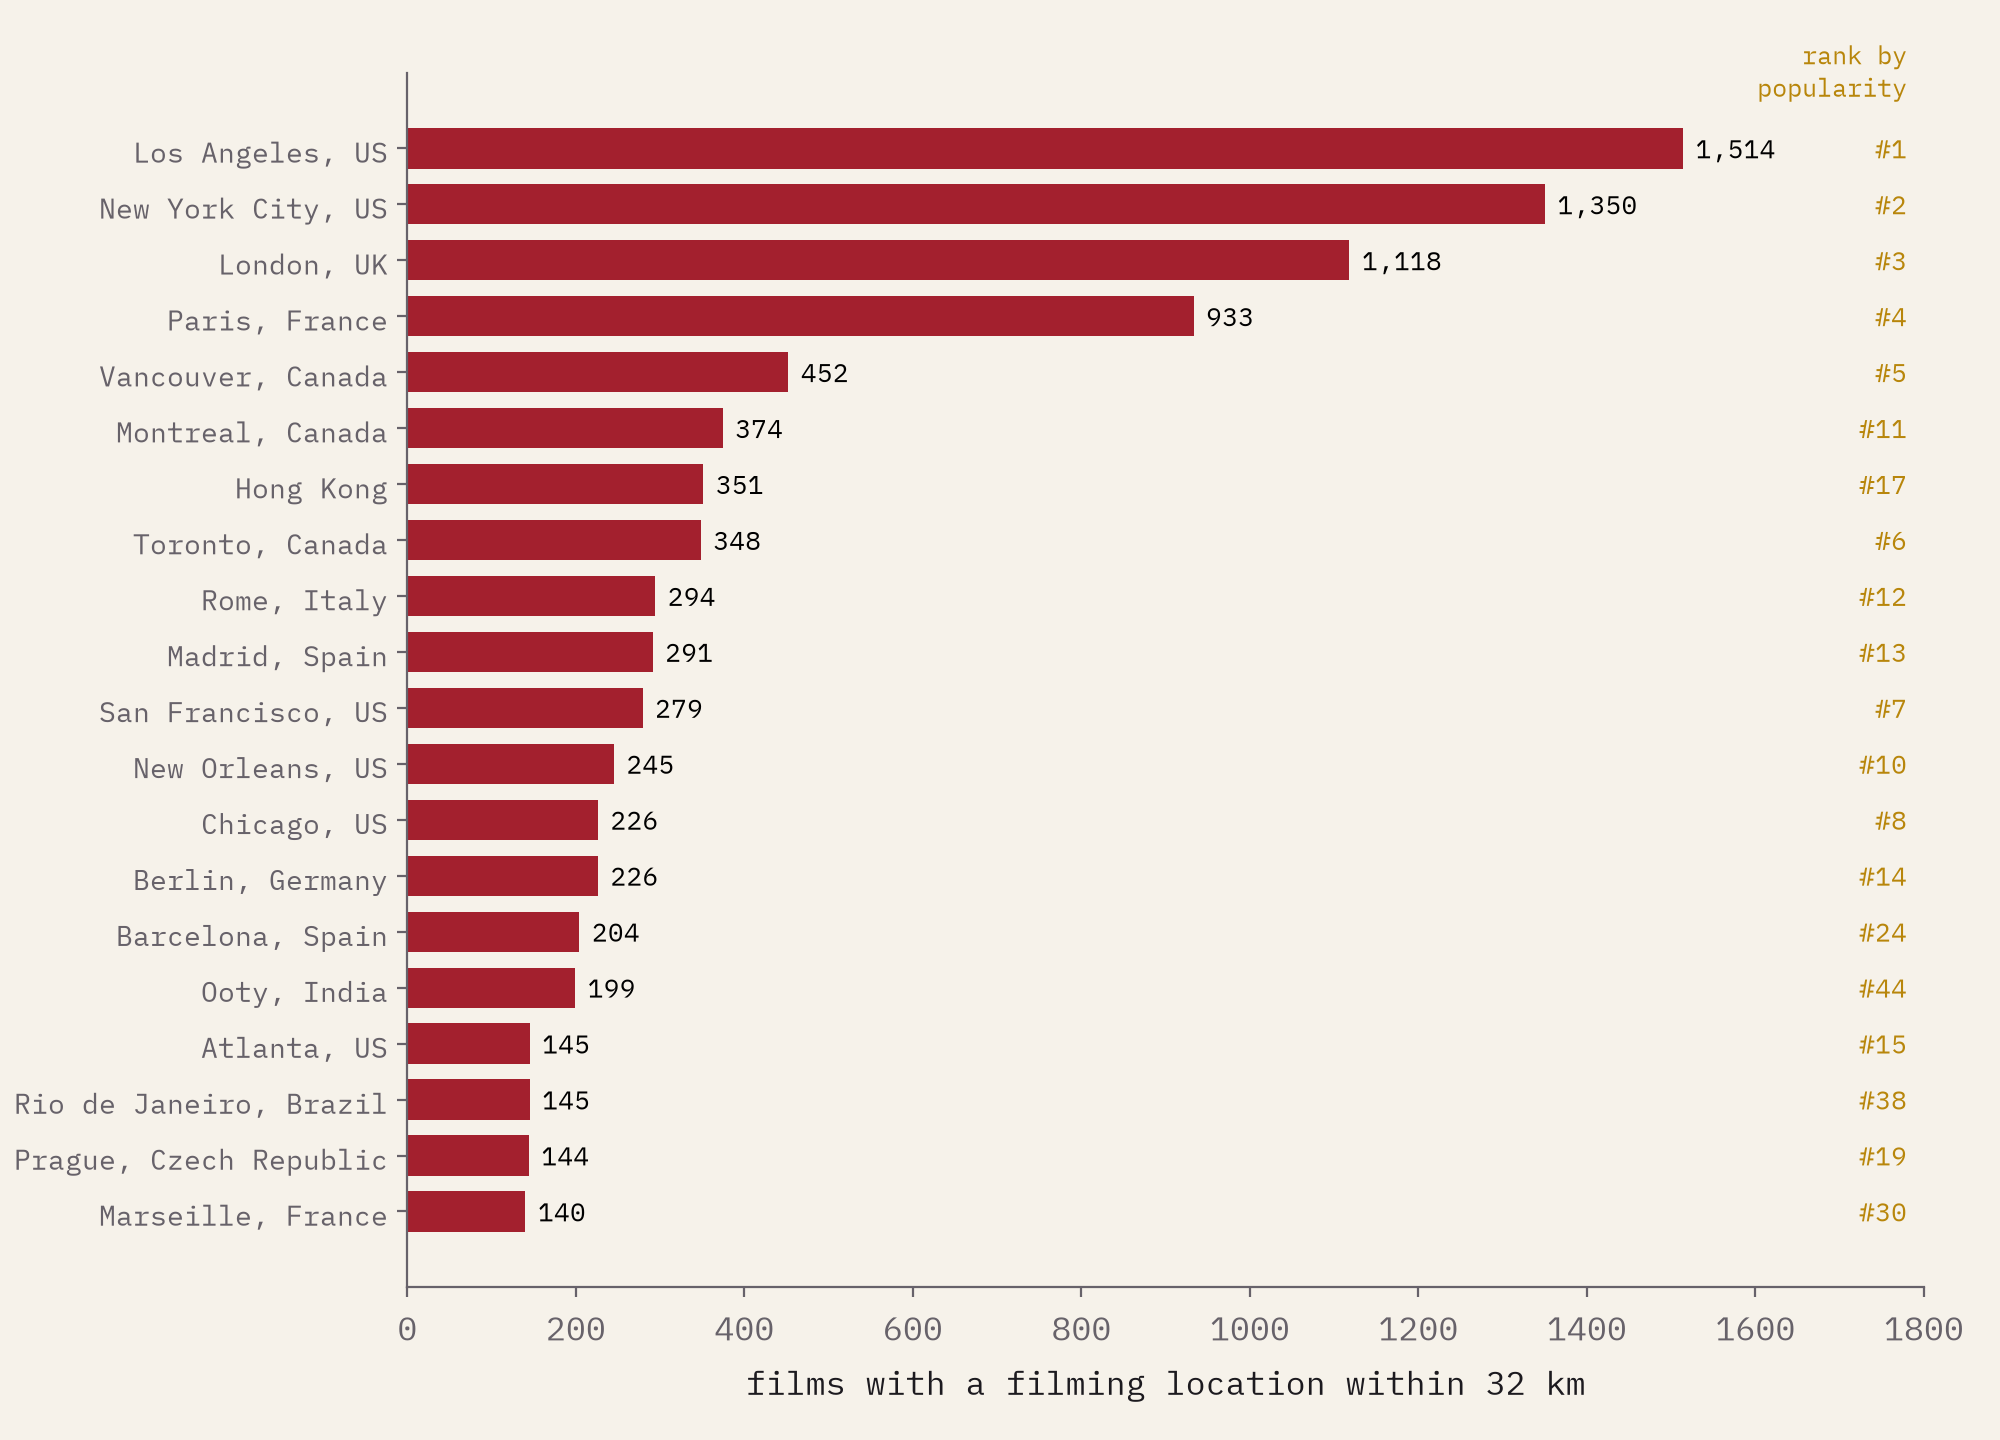
\includegraphics[width=.88\textwidth]{f_cities.png}
\caption{The twenty filming cities with most films, and (right, gold) their rank when films are weighted by sitelinks.}\label{fig:cities}\end{figure}

\subsection{Home and abroad}
Of 23,239 films with an origin and a located place, 4,329 (19\%) were shot at least partly abroad, 21\% excluding Indonesian films; 2,968 were shot only abroad. Table~\ref{tab:hosts} and Figure~\ref{fig:hosts} show the host countries. Canada hosts 717 foreign films, 95\% American, and is followed by the United States (292), the United Kingdom (287), France and Spain. In proportion, Malta (96\%), Morocco (82\%), Bulgaria (79\%) and Iceland (78\%) are filmed mostly by others. Large producers mostly stay home: only 4\% of films shot in the United States are foreign. Leaving home is commoner for British (32\%) and Indian (35\%) films than for American (25\%) or French (21\%) ones.

\begin{table}[tbp]\centering\small\caption{Countries hosting most foreign productions: films with a known origin shot there, foreign productions, share, and main origins.}\label{tab:hosts}\begin{tabular}{lrrr>{\raggedright\arraybackslash}p{5.2cm}}\toprule Country & Films & Foreign & Share & Main origins\\\midrule
Canada & 2,167 & 717 & 33\% & United States 683, United Kingdom 56\\
United States & 6,959 & 292 & 4\% & France 67, Italy 46\\
United Kingdom & 1,362 & 287 & 21\% & United States 208, India 31\\
France & 1,719 & 253 & 15\% & United States 138, United Kingdom 61\\
Spain & 1,064 & 252 & 24\% & United States 122, United Kingdom 75\\
Mexico & 362 & 182 & 50\% & United States 159, France 18\\
Italy & 912 & 161 & 18\% & United States 92, United Kingdom 37\\
Thailand & 161 & 141 & 88\% & United States 63, India 25\\
Morocco & 159 & 131 & 82\% & United States 62, France 44\\
Czech Republic & 308 & 120 & 39\% & United States 63, Germany 27\\
Switzerland & 183 & 113 & 62\% & United States 41, France 24\\
Bulgaria & 137 & 108 & 79\% & United States 76, Germany 16\\
Germany & 591 & 102 & 17\% & United States 55, France 17\\
New Zealand & 225 & 97 & 43\% & United States 55, India 20\\
Austria & 167 & 92 & 55\% & United States 36, Germany 34\\
\bottomrule\end{tabular}\end{table}

\begin{figure}[tbp]\centering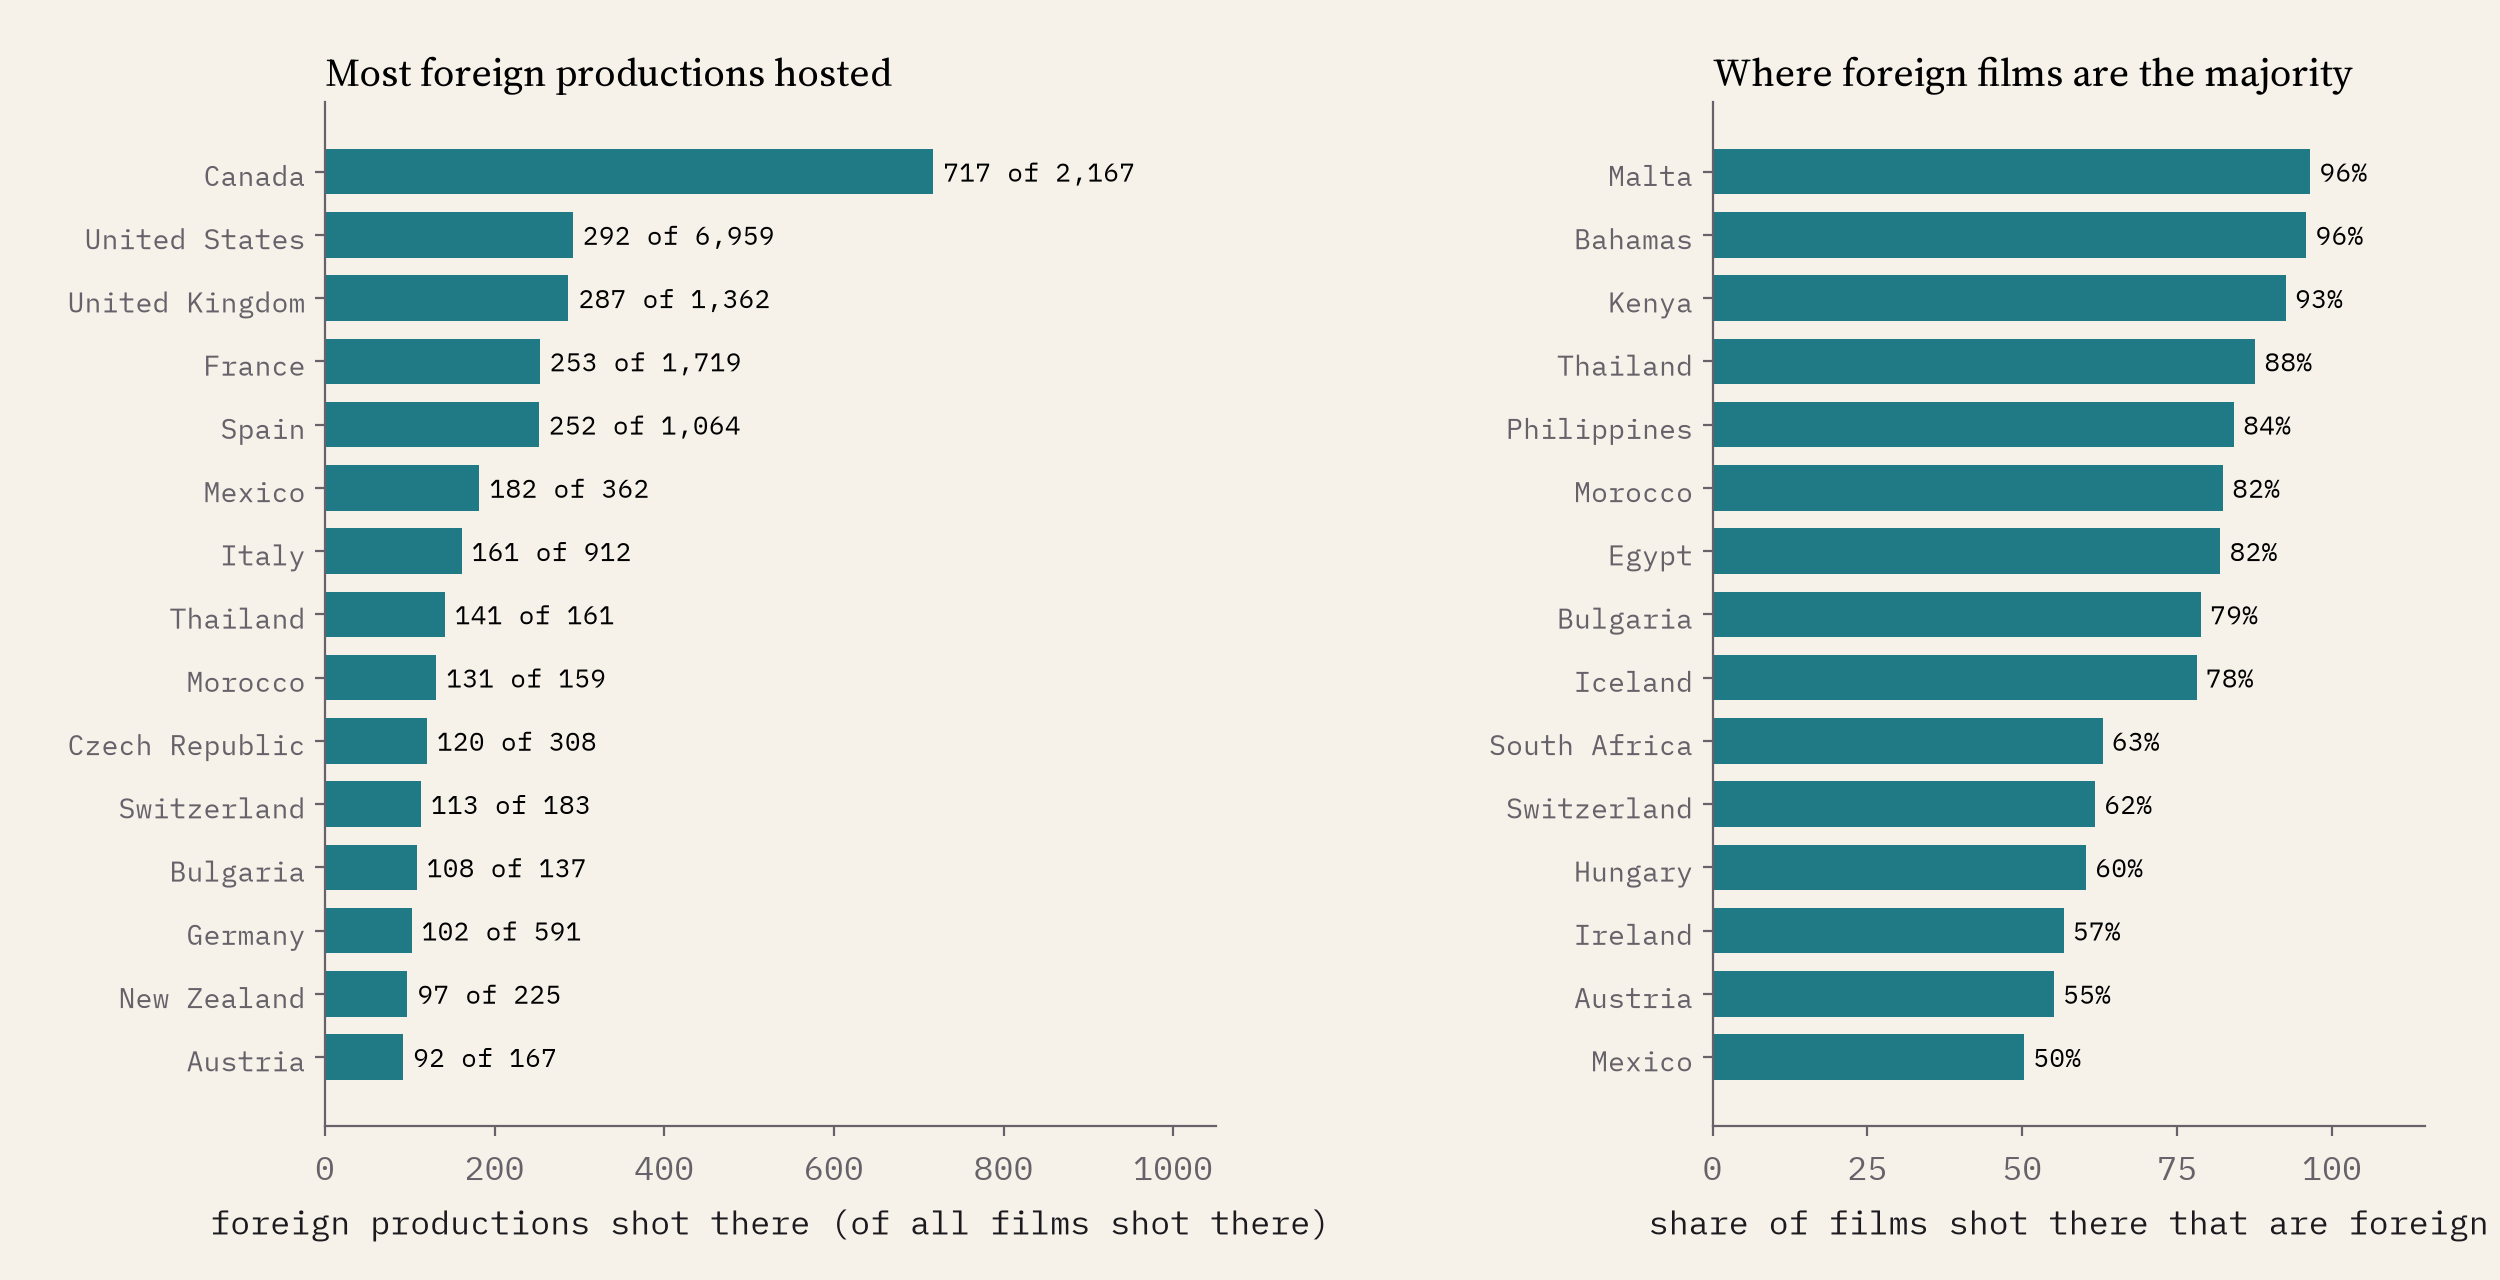
\includegraphics[width=\textwidth]{f_hosts.png}
\caption{Left: the fifteen countries hosting most foreign productions. Right: share of films shot in each country that are foreign, for countries with at least 40 films with a known origin.}\label{fig:hosts}\end{figure}

\subsection{Change by decade}
The share of films shot abroad rose from 20\% in the 1950s to 25\% in the 2000s and 24\% in the 2010s (Figure~\ref{fig:dec}). American films travelled early: 31\% of those from the 1960s were shot partly abroad. What changed more is the destination. Foreign productions in Spain peak in the 1960s, the era of European co-productions and westerns shot in Almer\'ia; Canada's in the 2000s, Bulgaria's in the 2000s and Hungary's and Iceland's in the 2010s. The 2020s run only to 2026 and are incomplete.

\begin{figure}[tbp]\centering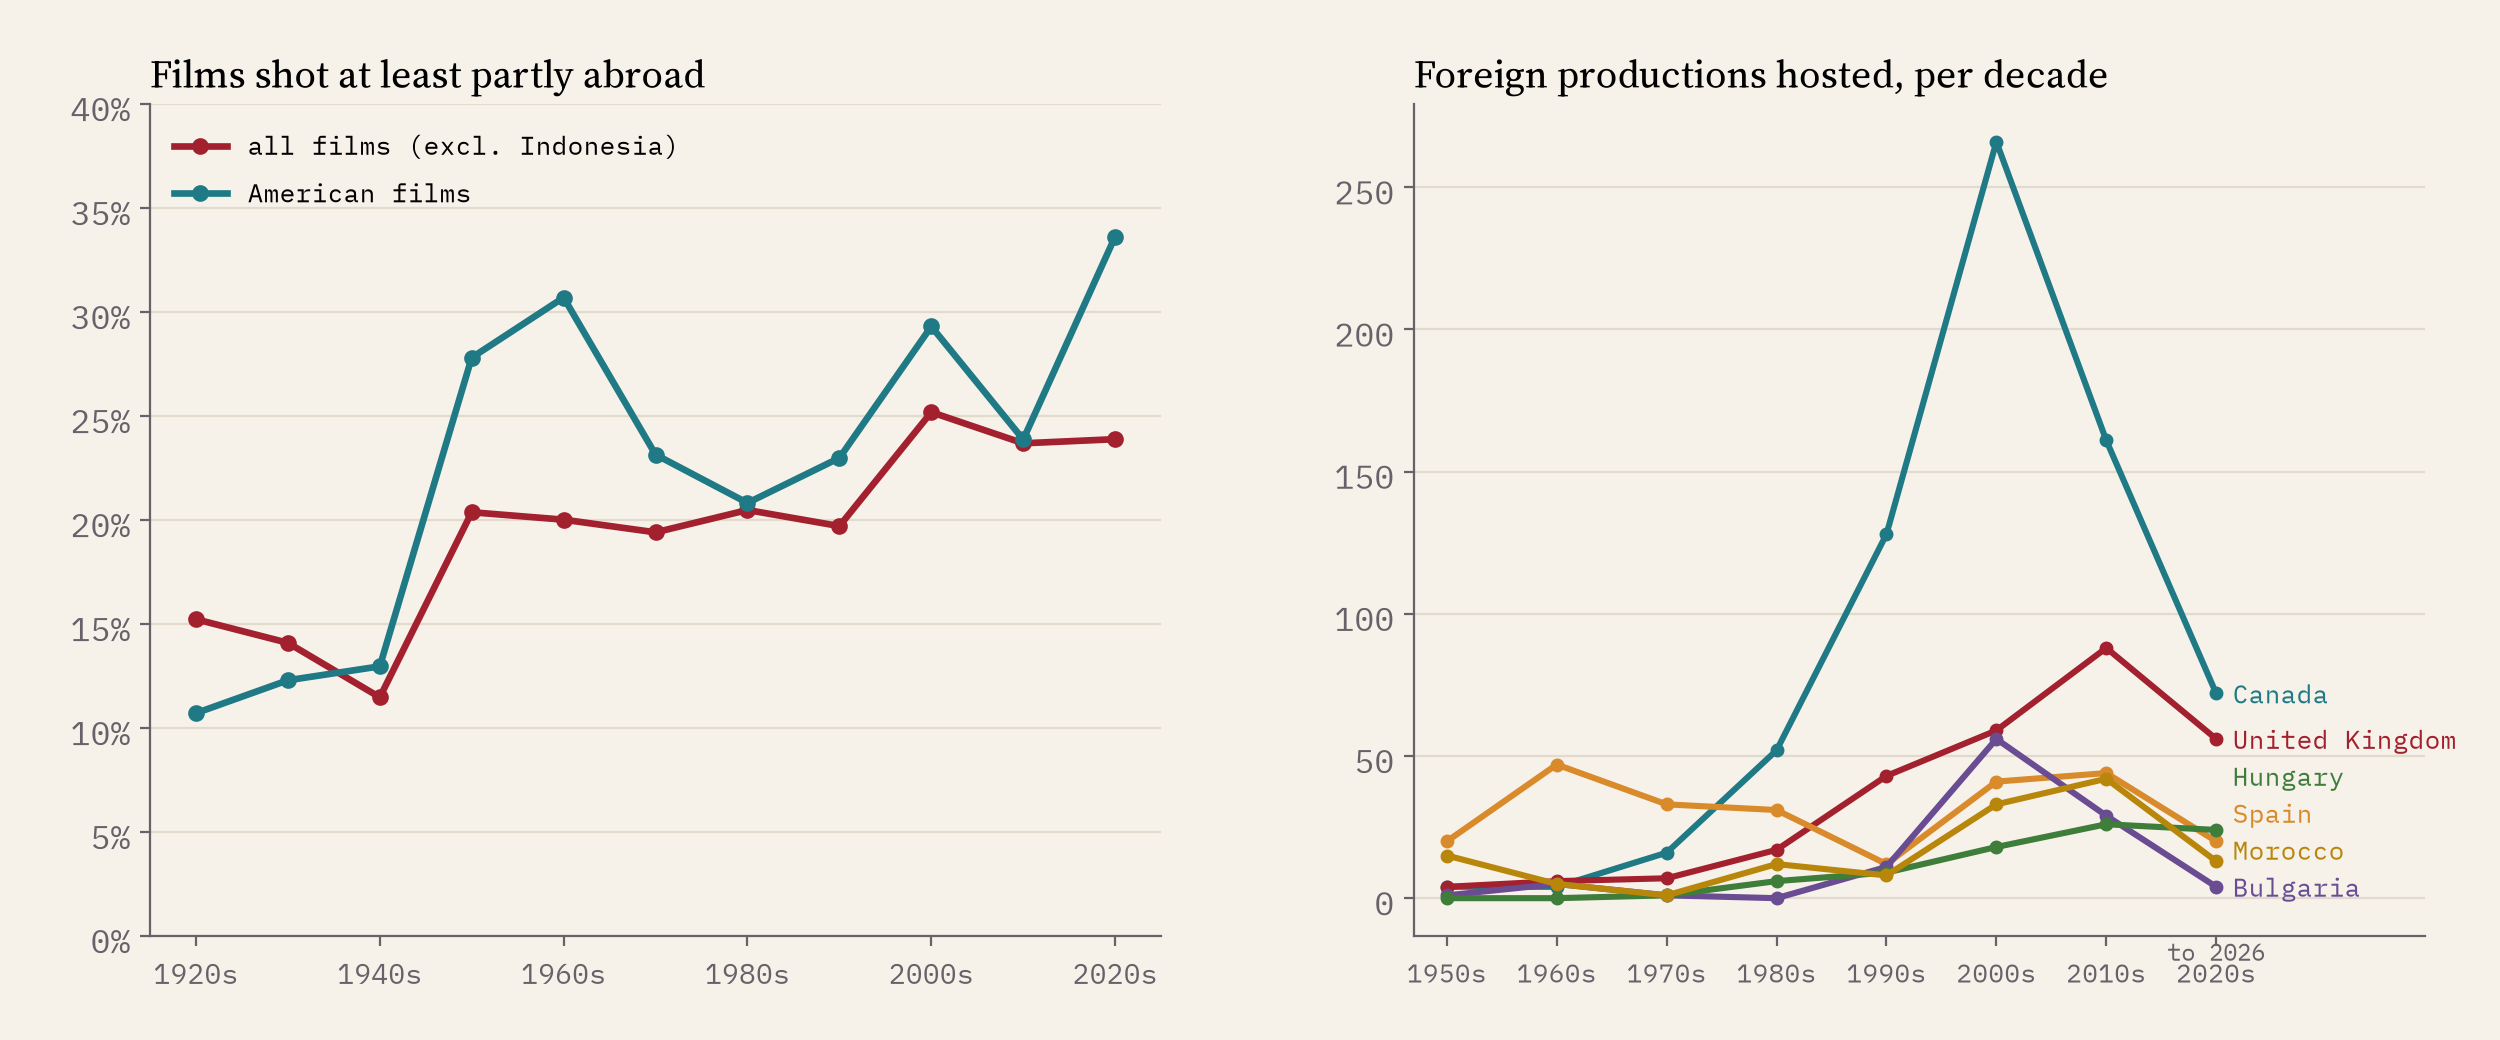
\includegraphics[width=\textwidth]{f_decades.png}
\caption{Left: share of films shot at least partly abroad, by decade. Right: foreign productions hosted per decade by six countries.}\label{fig:dec}\end{figure}

\subsection{Stand-in cities}
Among cities with at least 25 films with a known origin, foreign productions dominate in Valletta (96\%), Bangkok (85\%), Budapest (66\%), Vancouver (63\%) and Toronto (56\%) (Figure~\ref{fig:stand}). These are the cities known as stand-ins, but the data cannot confirm what they stood in for, since narrative location (P840) is not in the query. Several big host countries are recorded mostly at country level: 227 films were shot in New Zealand, but only 3 at a place in Wellington and 8 in Auckland.

\begin{figure}[tbp]\centering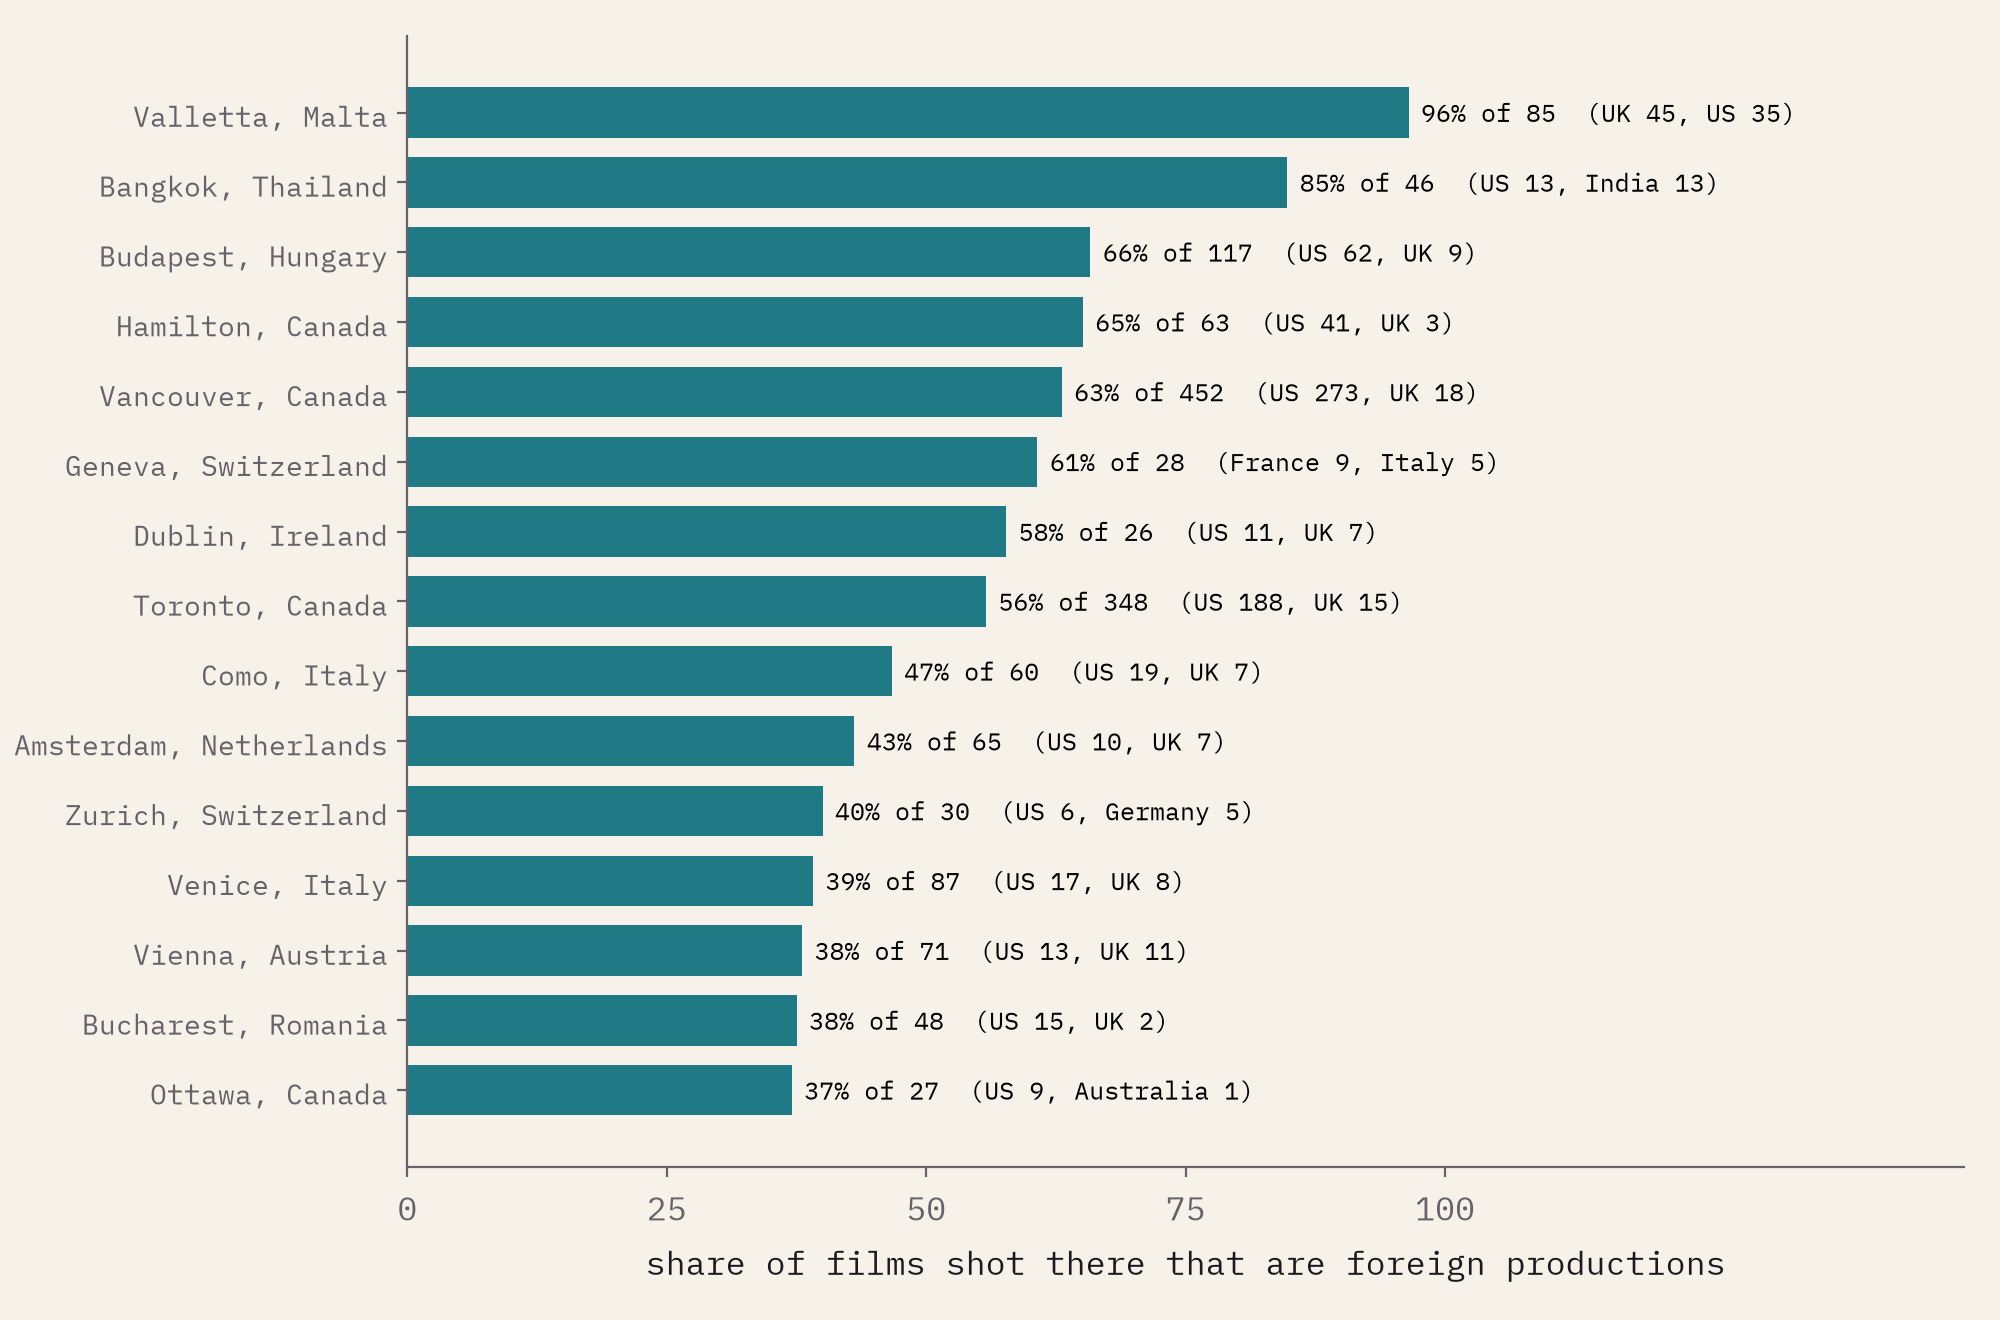
\includegraphics[width=.88\textwidth]{f_standin.png}
\caption{Cities where foreign productions are the largest share of recorded filming, with the two commonest origins.}\label{fig:stand}\end{figure}

\subsection{James Bond}
The 25 Eon films have 248 recorded locations, 179 distinct, in 36 countries and territories (Figure~\ref{fig:bond}, Table~\ref{tab:bond}). Pinewood Studios is listed for 22. After the United Kingdom the commonest countries are the United States (10 films) and Switzerland, Italy and the Bahamas (6 each). Documentation grows over time: films before 1990 average 6.6 locations, those since 2006 19.6; Spectre has 33 and Licence to Kill 2.

\begin{figure}[tbp]\centering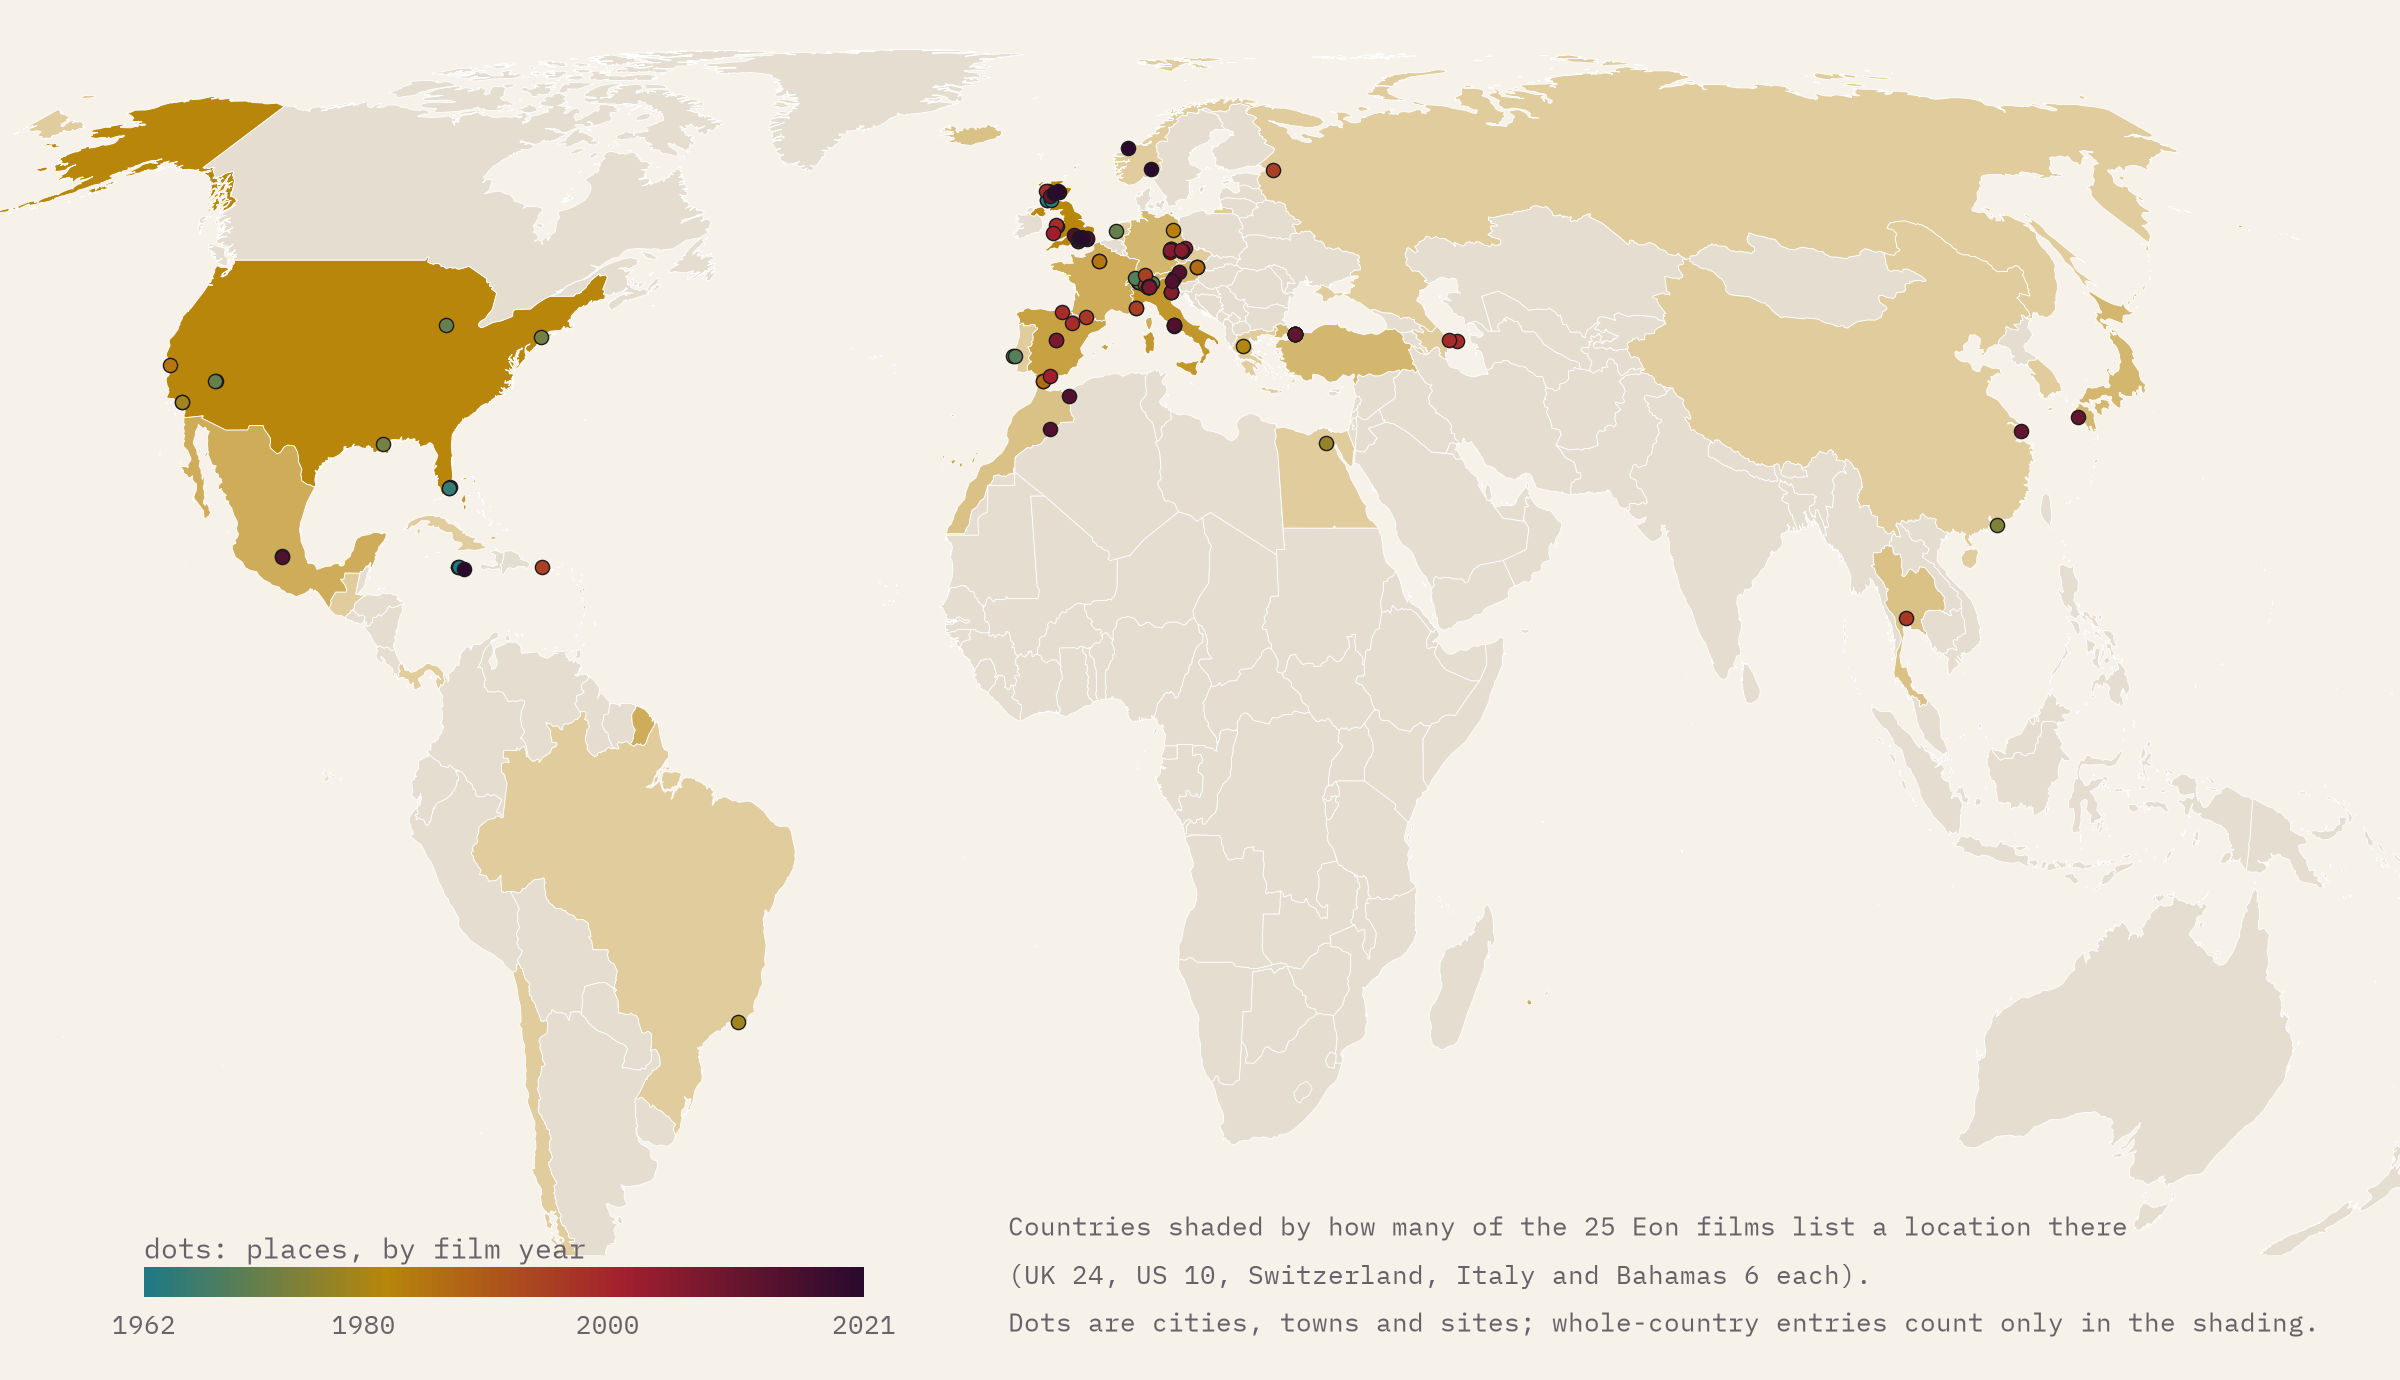
\includegraphics[width=\textwidth]{f_bond.png}
\caption{Filming locations of the 25 Eon James Bond films in Wikidata.}\label{fig:bond}\end{figure}

\begin{table}[tbp]\centering\footnotesize\caption{The 25 Eon James Bond films: recorded locations, whether Pinewood Studios is listed, and countries outside the UK.}\label{tab:bond}\begin{tabular}{rlrc>{\raggedright\arraybackslash}p{6.4cm}}\toprule Year & Film & Places & Pinewood & Outside the UK\\\midrule
1962 & Dr. No & 4 & yes & Jamaica\\
1963 & From Russia with Love & 18 & yes & Switzerland, Spain, Italy, Turkey\\
1964 & Goldfinger & 8 & yes & Switzerland, United States\\
1965 & Thunderball & 5 & yes & Bahamas, France, United States\\
1967 & You Only Live Twice & 5 & yes & Bahamas, Spain, Japan\\
1969 & On Her Majesty's Secret Service & 12 & yes & Switzerland, Portugal\\
1971 & Diamonds Are Forever & 9 & yes & Germany, Netherlands, United States\\
1973 & Live and Let Die & 3 & yes & United States\\
1974 & The Man with the Golden Gun & 3 & yes & Hong Kong, Thailand\\
1977 & The Spy Who Loved Me & 6 & yes & Bahamas, Switzerland, Egypt, Japan\\
1979 & Moonraker & 7 & yes & Brazil, Guatemala, Italy, United States\\
1981 & For Your Eyes Only & 5 & yes & Bahamas, Greece\\
1983 & Octopussy & 5 & yes & Germany, United States\\
1985 & A View to a Kill & 6 & yes & Switzerland, France, Iceland, United States\\
1987 & The Living Daylights & 8 & yes & Austria, Morocco, United States\\
1989 & Licence to Kill & 2 &  & Mexico, United States\\
1995 & GoldenEye & 13 &  & Switzerland, France, Monaco, Puerto Rico, Russia\\
1997 & Tomorrow Never Dies & 6 & yes & Germany, France, Mexico, Thailand\\
1999 & The World Is Not Enough & 17 &  & Azerbaijan, Bahamas, Spain, Turkey\\
2002 & Die Another Day & 8 & yes & Cuba, Spain, Iceland, South Korea, United States\\
2006 & Casino Royale & 29 & yes & Bahamas, Czech Republic, Italy\\
2008 & Quantum of Solace & 8 & yes & Austria, Chile, Spain, Italy, Mexico, Panama\\
2012 & Skyfall & 16 & yes & China, Japan, Turkey\\
2015 & Spectre & 33 & yes & Austria, Italy, Morocco, Mexico, Vatican City\\
2021 & No Time to Die & 12 & yes & Italy, Jamaica, Norway\\
\bottomrule\end{tabular}\end{table}

\subsection{Coverage}
The films come from 134 countries, but 40\% are American and 13\% Indonesian. India, the world's largest producer of feature films by number, has 614; China 197; Nigeria 13. Popular films are described in more detail: films with fewer than five sitelinks average 1.3 locations and 10\% were shot abroad, films with 50 or more average 3.6 and 44\% (Figure~\ref{fig:cov}). 78\% of films have a single recorded location.

\begin{figure}[tbp]\centering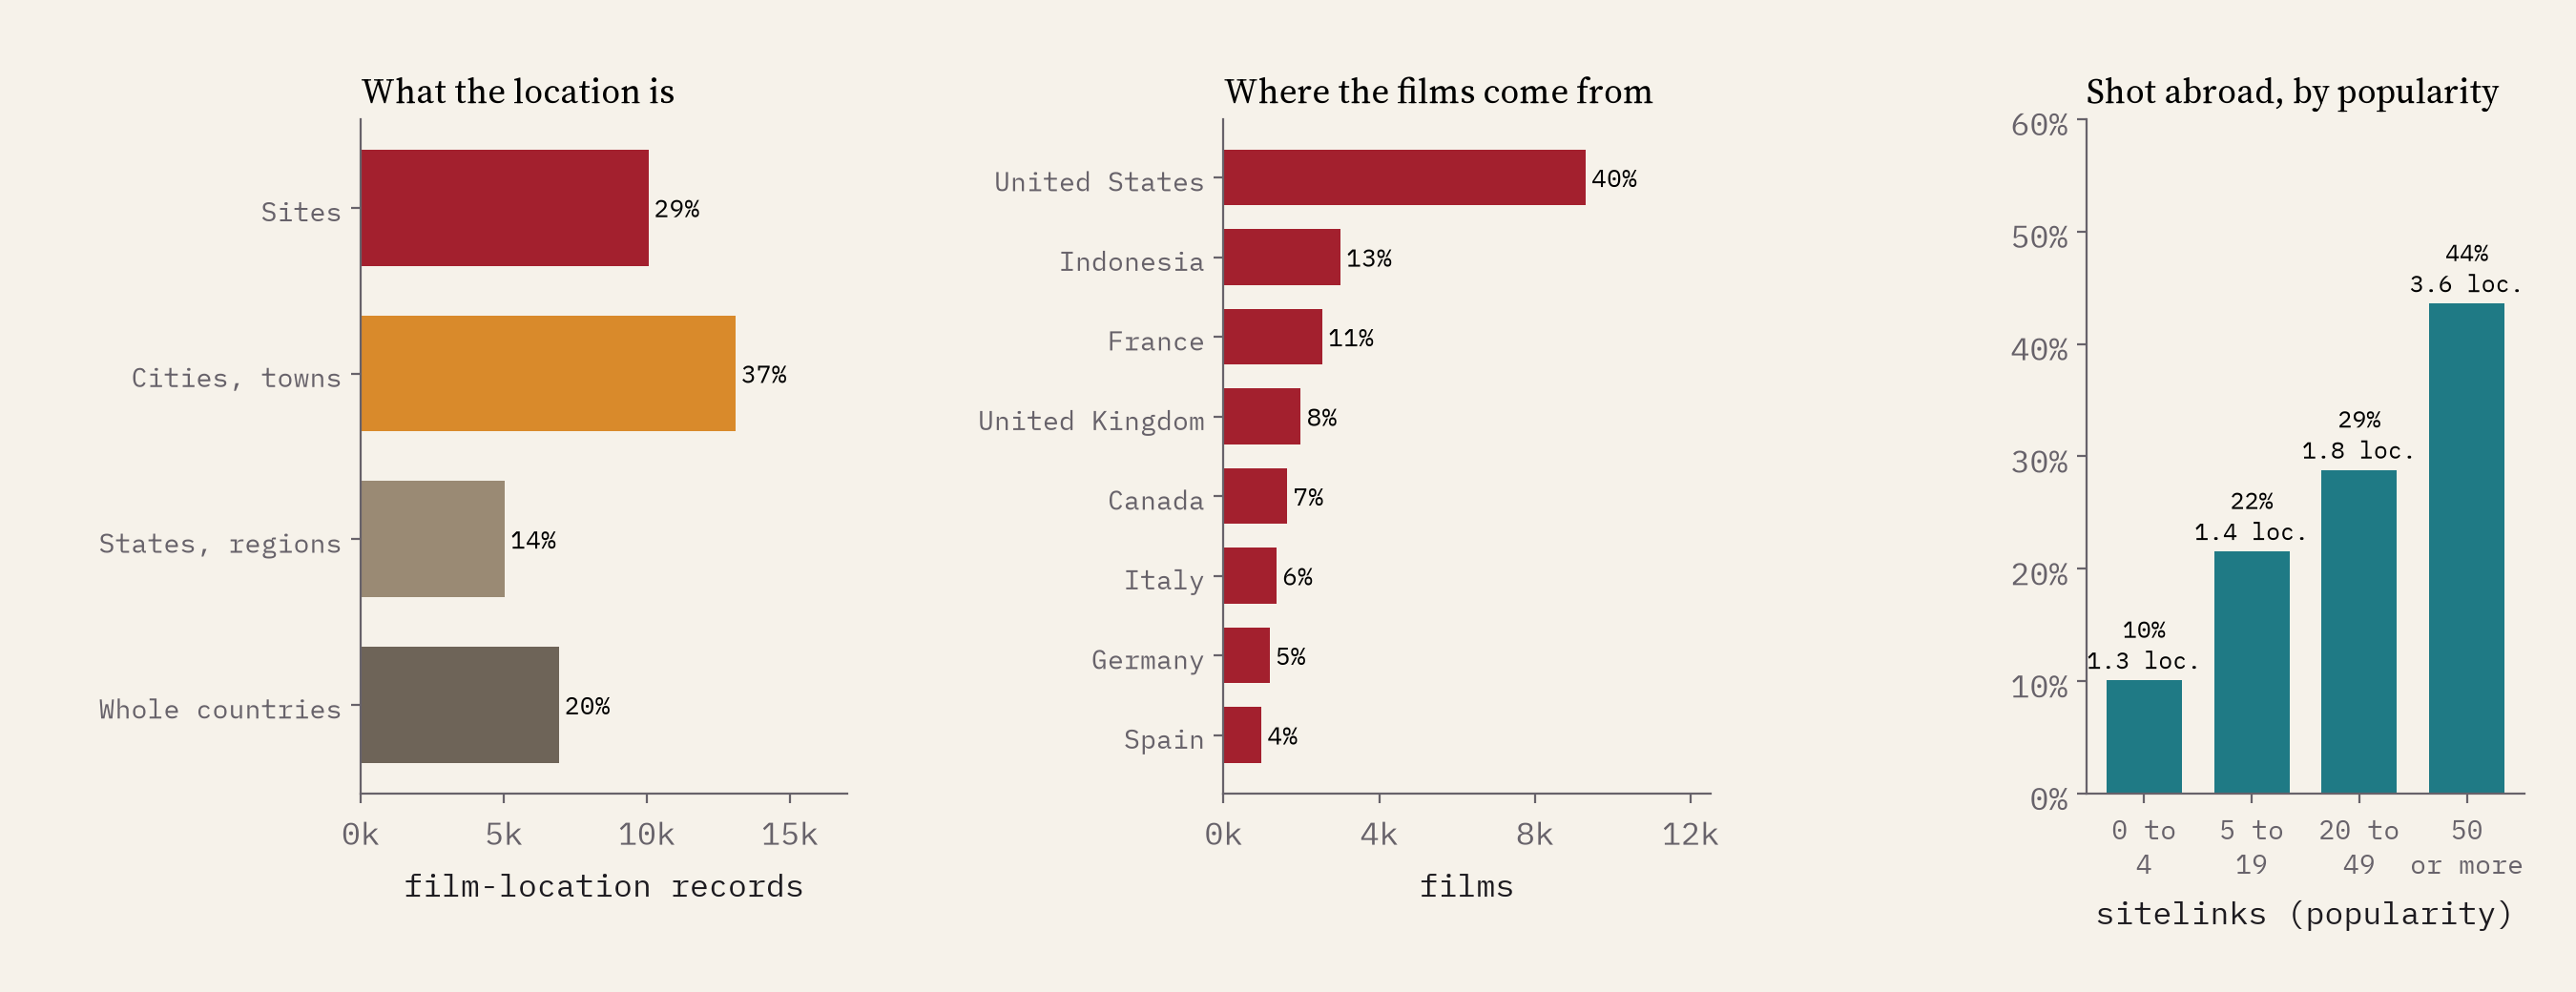
\includegraphics[width=\textwidth]{f_coverage.png}
\caption{Coverage: film-location records by level; films by country of origin; share shot abroad and mean recorded locations by popularity.}\label{fig:cov}\end{figure}

\section{Discussion}
Three features of the open record stand out. First, the concentration of filming in a handful of production cities, with Los Angeles, New York, London and Paris far ahead, matches what studies of film industry clustering would predict \citep{scott}. Second, the host-country pattern reflects the economics of runaway production: Canada's large count, overwhelmingly American, and the late rise of Bulgaria and Hungary are consistent with the role of tax incentives and studio building \citep{miller,goldsmith}. Third, and most important for interpretation, the record is shaped by who documents films. The rise in films shot abroad is partly a rise in recorded detail, as the Bond films show: earlier films travelled, but fewer of their locations have been entered.

\section{Limitations}
First, Wikidata's filming locations are incomplete and skewed to American, English-language and well-known films; totals count documented films, not films. Second, a third of film-location records name only a country or region; these are kept for country figures but cannot be mapped, so the point map understates places such as New Zealand and Morocco. Third, the level classification is rule based and will misclassify some locations, for example large islands treated as sites. Fourth, home and abroad depend on Wikidata's countries of origin, which for co-productions may list many countries and for others may be missing. Fifth, the data say nothing about setting, time on location or budget. Sixth, sitelinks measure Wikimedia attention, not audiences. Finally, all counts refer to one retrieval in 2026.

\section{Conclusion}
One open query is enough to draw a world map of filming, rank the film cities, show which countries host other countries' films and follow James Bond around the world. Its gaps are part of the result: the map shows where filming has been documented, and the interactive version lets readers see both.

\section*{Data and code availability}
The interactive map is at \url{https://maps.tristanhotham.com/film-locations/}. Data and code are at \url{https://github.com/Tristan-Hotham/film-locations} and archived with this paper at https://doi.org/10.5281/zenodo.23847354. Derived data are released under CC BY 4.0 and code under the MIT licence.

\section*{AI statement}
I wrote the text, with drafting and editing assistance from Claude (Anthropic), which also helped prepare the analysis code. I reviewed and checked all text and results.

\begin{thebibliography}{9}
\bibitem[Bast and Buchhold(2017)]{qlever} Bast, H. and Buchhold, B. (2017) QLever: a query engine for efficient SPARQL+text search. \emph{Proceedings of the 2017 ACM Conference on Information and Knowledge Management}, 647 to 656.
\bibitem[Goldsmith and O'Regan(2005)]{goldsmith} Goldsmith, B. and O'Regan, T. (2005) \emph{The Film Studio: Film Production in the Global Economy}. Lanham: Rowman and Littlefield.
\bibitem[Miller et al.(2005)]{miller} Miller, T., Govil, N., McMurria, J., Maxwell, R. and Wang, T. (2005) \emph{Global Hollywood 2}. London: British Film Institute.
\bibitem[Natural Earth(2026)]{naturalearth} Natural Earth (2026) Admin 0 countries, admin 1 states and provinces, and populated places. Public domain. \url{https://www.naturalearthdata.com/}
\bibitem[Scott(2005)]{scott} Scott, A. J. (2005) \emph{On Hollywood: The Place, the Industry}. Princeton: Princeton University Press.
\bibitem[Vrande\v{c}i\'c and Kr\"otzsch(2014)]{wikidata} Vrande\v{c}i\'c, D. and Kr\"otzsch, M. (2014) Wikidata: a free collaborative knowledgebase. \emph{Communications of the ACM}, 57(10), 78 to 85.
\end{thebibliography}
\end{document}
